\chapter{Introduction to Deterministic Methods}
\label{chap:determ_intro}

\epigraphhead[10]{\singlespacing
    \epigraph{
        Au milieu de l'hiver, j'ai découvert en moi un invincible été.
    }
    {Albert Camus}
}

This chapter provides more specific background and introduction to deterministic radiation transport methods.
I discuss the state of the art in deterministic radiation transport on GPUs and the various numerical methods needed to solve the four independent variable particle integro-differential equation implemented in this work.
I also summarize manuscript Chapters \ref{chap:therefore_paper} and \ref{chap:smom_paper} and their relationship to my research questions from Section \ref{sec:research_qustions}.

\section{S$_N$ approximation in angle}

There are two major methods of treating the double integral over all angles in Eq.~\eqref{eq:fullNTE}.
The method of spherical harmonics or P$_{N}$ method takes angular moments of the transport equation then makes a closure assumption at the N\ths  order.
This work focuses on the S$_N$ or discrete ordinance approximation, which turns Eq.~\eqref{eq:fullNTE} into a coupled (simultaneous) set of linear partial differential equations in each angular direction using quadrature integration.
It was first formulated by Chandrasekhar in the 1930s to describe radiative heat transfer in stellar media \cite{chandrasekhar1960radiative}.
The S$_N$ approximation was soon applied to neutron transport by Carlson \cite{precise1971carlson}, Lee \cite{discrete1961lee}, and Lathrop \cite{discrete1966lathnrop} with its earliest published description in 1953 \cite{carlson_1955_sn}.
The method of discrete ordinance was also adapted to general radiative heat transfer by Fiveland \cite{three1988fiveland} and Truelove \cite{discrete1987truelove}.

At this point it becomes necessary to describe the other governing assumptions I use in this work including:
slab geometry (1D-rectilinear coordinates), isotropic scattering and sources, as well as the multi-group assumption in energy distribution.
The methods I develop in this work are not restricted by these assumptions---and future work may explore the methods described here in anisotropic distributions in angle and/or solutions on unstructured meshes---but are made here for simplicity.
In fact, I make specific decisions in this work with the underlying discretization schemes to allow for eventual extension to these regimes.

When applied to Eq.~\eqref{eq:fullNTE} the resulting initialization point is described by
\begin{multline}
    \label{sn_nte_int}
    \frac{1}{v_g} \frac{\partial \psi_{m,g}(x,t)}{\partial t} + \mu_m \frac{\partial \psi_{m,g}(x,t)}{\partial x} + \Sigma_g(x) \psi_{m,g}(x,t)  \\
     = \frac{1}{2} \left( \sum\limits_{g' = 0}^G \Sigma_{s, g'\to g}(x) \sum\limits_{n=1}^N w_n \psi_{n, g'}(x,t) + Q_g(x,t) \right) \;, \\
    \qquad g=1 \ldots G \;, \qquad m=1 \ldots N \;, \qquad t > 0 \;, \qquad x \in [0,X] \;,
\end{multline}
where $\psi$ is the angular flux, $x$ and $t$ are independent continuous variables for 1D space and time respectively, $X$ is the spatial width of the problem, $g$ is the group index, $G$ is the total number of energy groups, $v$ is speed, $w$ is an angular quadrature weight, $\mu$ is the angular quadrature ordinate ($\cos(\hat{\Omega}_\theta)$), $m$ is the quadrature index, $N$ is the total number of angles in quadrature, and $Q$ is the isotropic material source.
In this work I will exclusively use Gauss-Legendre quadrature, but if extended to higher dimensions other quadratures sets would be required to evaluate the double integral over both angular directions (e.g., level-symmetric). 
The initial and boundary conditions are again prescribed angular flux distributions:
\begin{equation*}
    \psi_{m,g}(x,0) = \psi_{m,0}(x), \qquad m=1 \ldots N \;,
\end{equation*}
\begin{equation*}
    \psi_{m,g}(0,t) = \psi_{m,L}(t), \qquad \mu_m >0 \;,
\end{equation*}
\begin{equation*}
    \psi_{m,g}(X,t) = \psi_{m,R}(t), \qquad \mu_m <0 \;.
\end{equation*}
Via the multi-group assumption and S$_N$ approximations there are $NG$ partial differential equations to solve.
From here additional discretization can be used to turn the continuous functions of angular flux, source, material data, and differential operators into numerical approximations.

\section{Time-space discretization schemes}

To enable this work in both space and time, discretization schemes are needed to treat the differential operators and continuous functions.
%As the goal of the research is for development on heterogeneous architectures, communication to work ratio may become an issue.
When solving equations on the GPU, numerical algorithms that require lots of communication back and forth between the host (CPU) and device (GPU) will limit the maximum allowable performance for many GPU accelerators.
To abate this issue, higher (second) order discretization schemes can be used to add to the compute work required in every iteration, thus improving the communication-to-work ratio.

Various classes of spatial discretizations can be used in radiation transport.
Finite difference, finite element, and finite volume methods are all often employed with the most common in radiation transport being diamond-differencing ($\mathcal{O}(2)$).
Diamond-difference is popular as it is the only second-order space discretization that uses a single interior (cell-averaged) degree of freedom; however it only works on orthogonal grids.
%Intended future investigation of the scheme in this research are into non-uniform meshes.
To allow future work to more readily extend the algorithms described here to unstructured grids I make specific decisions about a discretization scheme---in other words, not diamond-differencing.
Instead I use a scheme specifically designed for use on unstructured grids called corner-balance method, which was originally developed by Adams~\cite{adams_subcell_1997}.
Specifically I use the \emph{simple} corner balance ($\mathcal{O}(2)$) which is a a finite volume method thus it enforces conservation within sub-cell volumes in a spatial cell.
Simple corner balance was determined to be sufficient as it is higher  order.
%Simple corner blance is not acrurate in the thin-limit however a slight alteration to it 
Simple corner balance is equivalent to the lumped-linear discontinuous finite element method in 1D.
%This spatial discretization is similar to what has been implemented in both iterative algorithms explored in this work.

%Solving the transport equation with deterministic methods typically involves iterative schemes to converge the scattering source and transport operators (this is discussed more in section \ref{sec:intro_itterative-scheme}).
To treat the continuous operators in time, implicit time marching schemes are often used as they have desirable stability properties.
Specifically, implicit (backward) Euler ($\mathcal{O}(1)$) or Crank--Nicolson ($\mathcal{O}(2)$) \cite{nicolson_phd, Crank_Nicolson_1947} are the most often employed.
%These schemes are advantageous as they often act like a wrapper around a steady state deterministic transport solver with few changes needed to implement.
While Crank--Nicolson is second-order accurate, it is not robust and can produce negative solutions and spurious oscillation.
Time-dependent version of the multiple balance approach was derived by Variansyah, Larsen, and Martin~\cite{variansyah_robust_2021, ilham_phd} to be a robust, higher ($\mathcal{O}(2)$) order time discretization scheme.
The multiple-balance method was originally developed as a space discretization scheme.
The full space-time-energy-angle discretization scheme is derived in chapter \ref{chap:therefore_paper}. % and is explicitly shown in Equations \eqref{eq:scatter_mg} and \eqref{eq:fullOCI_mg}.

\section{Iterative Methods}

The linear system of equations formed by the space-energy-time-angle discretization scheme described in the previous sections can be posed as
\begin{equation}
\label{eq:introaxb}
    {A}x=b \; ,
\end{equation}
where $x$ is generically a dependent quantity of interest, and specifically in this work it is angular flux ($\psi$). 
This linear system of equations may be solved directly (e.g., LU decomposition with pivoting) or iteratively (e.g., Jacobi or Gauss--Seidel iterations).
The dimensions of these problems are \emph{huge} and \emph{sparse}, going by the number of:
\begin{itemize}
    \item angles in quadrature: \num{2}--\num{100};
    \item energy groups: \num{1}--\num{100};
    \item sub-cell discretizations: 4; and
    \item spatial cells: which can be hundreds up to millions for 1D problems.
\end{itemize}
This is the impact of the curse of dimensionality and is only further compounded when moving to higher spatial dimensions. 
Direct simulations are often prohibitively memory and computationally expensive.
Most often in production codes these systems are solved with some kind of iterative scheme.

To solve the discretization system iteratively, a fixed point (or Richardson) scheme is often used.
These are a broad class of iterative methods where \emph{old} information (from the immediately previous iteration) is used to form a new right hand side, which in turn is re-solved for a new estimation of the quantity of interest.
A fixed point iteration requires the system to allow for the dependent variable to exist on either side of the equality.
This is done with \emph{operator splitting}, specifically matrix splitting.

For example consider a splitting of Eq.~\eqref{eq:introaxb}, where $A = C+B$. $x$ acts on \emph{both} $C$ and $B$, so $x$ can be distributed such that the new system is
\begin{equation}
    Cx + Bx = b \; .
\end{equation}
Seemingly this has done nothing but further complicated the linear system.
Here's the kicker: the information multiplying one of these systems (lets say $B$) is initially \emph{guessed}, call it $x^{(0)}$.
Moving this known vector quantity to the right hand side gives
\begin{equation}
    Cx = b - Bx^{(0)} \; ,
\end{equation}
where the right hand side is now a known vector.
This equation is in the same form as Eq.~\eqref{eq:introaxb} and can be solved in the same way for a \emph{new} version of $x$!
This new value can then be reinserted back into the right hand side and used to recompute a new-new version of $x$.
Writing this for any generic iteration gives
\begin{equation}
\label{eq:introopsplit}
    {C}x^{(l+1)} = b - Bx^{(l)} \; ,
\end{equation}
where $l$ is the iteration index.

On the first iteration the dependent variable is either guessed, estimated, or (if running a time-dependent problem) the converged solution from the previous time step.
The iteration will continue until the quantity of interest stops changing between iterations: when the scheme has \emph{converged}.

There are other classes of iteration schemes. 
The most common is GMRES (\textbf{G}eneralized \textbf{M}inimal \textbf{RES}idual method), which is a more clever way of determining an \emph{optimal} guess at the beginning of each iteration.
GMRES keeps solutions of the dependent variable at multiple iterations and finds a guess that is orthogonal to previous guesses \cite{kylov2004warsa, subspace2004warsa, gmres1996kelley, patton_gmres_2002}.
In effect it is a way of analyzing how the solution is chaining iteration-to-iteration then picking a new starting point at a location that is interpolated to be the closest to a \emph{converged} solution.
Newton iterations are another solver technique that uses information about the derivatives of the systems with respect to their independent variables to solve for a new guess \cite{ctkelle_newton}.
This work focuses on fixed point iterations, but other iteration schemes could be explored for future work.

The process of separating components of the dependent variable to either side of an equation, letting one lag, and solving for an update is called \emph{operator splitting}.
The specifics of a given operator splitting will determine the organization of the linear systems in $\bm{A}$ and $b$, which in turn will determine how they can be efficiently solved within each iteration (to get $x^{(l+1)}$) and what tools can be used to implement those solvers (more on this in sections \ref{c2:source_iterations} and \ref{c2:oci}).
The operator splitting will also impact how many iterations it will take to reach convergence (more on this in sections \ref{c2:precon} and \ref{c2:specrad}).
For high fidelity problems these systems are still massive, and require their solution to be computed in parallel on modern high performance computers.


\subsection{Eigenvalues and the Spectral Radius}
\label{c2:specrad}

Eigenvalues are useful to measure the behavior of numerical and physical systems as they evolve with respect to some independent variable.
In its most pure form, an eigen-system (with eigenvalues and vectors) describes how a repeated process impacts the elements of a matrix ($T$) and takes the form
\begin{equation}
    {T}v = v\lambda \;,
\end{equation}
where $v$ are the eigenvector and $\lambda$ is an eigenvalue \cite{isaacson_numerical_1966, golub_matrix_1983}.
For systems of differential equations eigenvalue analysis can be used to identify scales on which quantities of interest are varying in order classify \emph{stiffness} \cite{niemeyer_phd, walker_phd}.
Eigen-systems can be used to classify and analyze oscillatory behavior including mechanical vibrations \cite{liang_vibrations}, sound \cite{howle_2001_eigenvalues}, and quantum mechanical processes \cite{maggie_phd, krane_2019_modern}.
In nuclear systems (or any population model) eigenvalues can describe the growth or decay of the total neutron population and thus the \emph{criticality} of the system \cite{duderstadt_hamilton, trahan_phd}.
Eigenvalue systems are often used when analyzing numerical methods to understand how error propagates as numerical schemes iterate.

In this work I use eigenvalues to describe how error of a dependent quantity of interest is propagated by either time stepping \cite{ilham_phd} or by iterative solution method like one described in the previous section \cite{southworth_phd}.
For the former eigenvalues can measure stability, and prove that a given space-time discretization scheme is {unconditionally stable} \cite{Lax_1956_stability}.
If all eigenvalues are below a certain threshold the compounding effect of error incurred at every time step will remain bounded.
For the latter the eigen-spectrum of the iteration system formed by operator splitting and preconditioners can measure convergence rates.

As an example of error propagating through an iterative method consider Eq.~\eqref{eq:introopsplit} reformed to describe how the error changes iteration to iteration
\begin{equation}
    f^{(l+1)} = {T}f^{(l)} \; ,
\end{equation}
where
\begin{equation}
    {T} =   A^{-1}B \;,  %\bm{A}^{-1}b \; .
\end{equation}
and $f^{(l)} = x^{\text{converged}} - x^{(l)}$ is the error between the converged true solution of the system and the estimation provided at iteration $l$.
${T}$ is applied to the quantity of interest (in this case error) over and over and over again as the iteration progresses.
So reforming the iteration as
\begin{equation}
    f^{(l)} = {T}^{l}f^{(0)} \; ,
\end{equation}
where $x^{(0)}$ is the initial guess and ${T}^{l}$ is raising ${T}$ to the $l$\ths power.
In this form it is apparent that the iteration is doing the same thing to a square matrix over and over again.
The concept is the same for time stepping as each time step is the reapplication of the same square time-stepping matrix, providing constant properties at time step size.
%To solve practical problems $T$ is never compute the as the order of the system is to big to analytically or numerical invert. % and we don't know the structure of $T$ as it requires a priori information about the solution which we only have for problems known anaclitic solutions.
%So analysis is limited to model problems, for radiation transport often the infinite homogeneous pure absorber.

Deriving $T$ is often done with von Neumann stability analysis, also known as Fourier stability analysis on a model problem\footnote{For radiation transport the simple model problem is often the infinite homogeneous medium problem.} \cite{leveque2007finite}.
The error on a given discretization stencil is expanded in a series of temporal or spatial Fourier modes, where each mode has a coefficient, an amplitude ($\lambda$), and a shape function (commonly $e^{i\omega x}=\cos{\omega x} + i\sin{\omega x}$).
The amplitude is the eigenvalue at a given frequency $\omega$.
As this is a sinusoidal system all the eigenvalues can be considered bounded $\omega \in [0, 2\pi]$.
Once $T$ is constructed, a solver from a linear algebra library can be used to compute it's eigenvalues ($\lambda_T$)\footnote{e.g., From LAPACK's GEEV algorithm \cite{laug}}.
Using these eigenvalues we can define the domination eigen value as
\begin{equation}
    \rho \equiv \sup_{\omega\in[0,2\pi]}\left|\lambda_T\right| \; ,
\end{equation}
the spectral radius.

John Crank and Phyllis Nicolson briefly described this method of analysis in 1947 while investigating the stability of numerical methods for solving the heat equation \cite{nicolson_phd}.
Their work would later become the Crank--Nicolson method \cite{Crank_Nicolson_1947}.
Charney, FjÖrtof, and von Neumann later described the method in greater detail while studying vorticity in the Earth's atmosphere in 1950 \cite{charney_1950_stabilityAnylisys}\footnote{The numerical experiments in \cite{charney_1950_stabilityAnylisys} were only possible by the efforts of programmers of the ENIAC computer, including Norma Gilbarg, Ellen-Kristine Eliassen, and Margaret Smagorinsky \cite{switman_2017_unheralded}}.

To ensure a time stepping scheme is unconditionally stable
\begin{equation}
    \rho \leq 1.0 \; ,
\end{equation}
which is the {von Neumann stability criterion} which in turn is related to the {Lax-Richtmeyer} equivalence theorem.
%This equation is for the maximum of the absolute values (eigenvalues can be complex and/or negative) of the eigenvalues to be less then or equal to one.
The eigenvalues measure how much error is increasing through time, so if the biggest or dominant one is less than one in magnitude, the error is bounded.
If it is greater than one, then the error will grow exponentially time step to time step.
Notably, ${T}$ will contain the time step size so this analysis can be repeated at various time steps sizes.

For an iterative method to be stable
\begin{equation}
    \rho < 1.0 \; .
\end{equation}
For an iterative scheme to be convergent it must be wholly less than unity---error must be decreasing iteration to iteration.
Furthermore, as $\rho$ gets smaller between $[0,1)$, the iteration converges faster.
Again the The spectral radius measuring how a value changes through a repeated process, only here it's iteration to iteration.
In this case $T$ will have information about scattering, total absorption, and spatial discretization so the spectral radius can be evaluated over a parameter space (see Chapter \ref{chap:therefore_paper} and Appendix \ref{chap:spec_rads}).
The spectral radius can be empirically measured by any transport solver by computing
\begin{equation}
    \rho_e = \frac{\left|\left|x^{(l+1)} - x^{(l)}\right|\right|_{2}}{\left|\left|x^{(l)} - x^{(l-1)}\right|\right|_{2}} = \frac{\text{error}^{(l+1)}}{\text{error}^{(l)}} \; .
\end{equation}
Effectively $\rho$ is the ratio of subsequent residuals.
This could be done to control false convergence, trigger in-situ algorithmic adaptions, or verify the implementation of a transport solver against anaclitic Fourier analysis, as they should match when running the same problem.

One thing to note is that the spectral radius is defined as the absolute value.
However, the dominant eigenvalues which actually govern convergence behavior may be complex.
In this work I found that the dominant eigenvalues may have significant complex components from both choices of time stepping scheme \cite{ilham_phd, ilham} and as a consequence of an iterative method.
This impacts convergence rate leading to oscillations in the residual and empirical measurements of spectral radius (see section \ref{sec:results-faoci} for more).

%This was very surprising and took a while to determine the reason was from these dominant eigen values as initially I thought I was just wrong.
While not a novel discovery \cite{anistratov_iterative_2015} this is one of the most interesting findings of this work from my own perspective.
This bucked my understanding of something I learned from numerical methods classes and written in textbooks:
that spectral radius \emph{governed} convergence and it is always real.
Appendix \ref{chap:spec_rads} shows plots of the entire eigenfunction of the two iteration schemes explored in this dissertation at various points in phase space.
The patterns they form are striking and beautiful.

\subsection{Source iteration}
\label{c2:source_iterations}

The source iteration (SI) method is a common operator splitting for the radiation transport equation.
The contribution to the solution from the scattering source (summation in the RHS of Eq.~\eqref{sn_nte_int}) is allowed to lag, while the angular flux is solved in every ordinate via transport ``sweeps" through the spatial domain \cite{lewis_computational_1984}.
It is often accompanied by preconditioners or synthetic accelerators (more on this in section \ref{c2:precon}) and GMRES.
SI sweeps in Cartesian geometries are readily parallelized over the number of angles, as the source term is known from the previous iteration, allowing the angular flux in each ordinate to be computed independently.
While any parallelization is a benifit to performance, a scheme that is embarrassingly parallel over the dimension with the greatest number of degrees of freedom---space---may be advantageous.
In a single spatial dimension SI is \textit{inherently serial} in space and cannot be parallelized.
In curvilinear geometries (e.g. spherical or cylindrical) other parallelism schemes may exist \cite{palmer_phd}.

In higher spatial dimensions, many S$_N$ production codes that implement SI use some kind of wavefront marching parallel algorithm also known as a Kockh--Baker--Alcouff scheme \cite{baker_kba_2017, colomer_parallel_2013} also called "full parallel sweeps" in literature.
In this scheme a sweep begins in a spatial location where all cell dependencies are known from boundary information (e.g., a corner).
From there on a hypothetical 2D grid, the two nearest neighbor cells are computed independently, potentially in parallel; the next step would be four cells.
This diagonally expanding wavefront continues to march and is able to better parallelize as many cells spatially as possible eventually saturating the number of work threads if the problem is large enough.
This may not be the most optimal to implement on GPUs (see Section \ref{sec:therefore_disscusion}).
%On CPUs this has been shown to be performant but this changing amount of work is not optimal on GPUs where.
%Performance evaluations of production codes that implement KBA on GPUs is sparse in literature and when avaliable is from proxy-apps.
%Ardra has such a proxy app 
%KBA algorithms are also tricky to efficiently implement in domain decomposed where wave front propagation between boundaries can be tricky.
%While this work is concerned with 1 spatial dimension when analyzing the state of the art it is important to consider that this is done.

%This has proven successful in modern transport applications on CPUs 
%(e.g., PARTISN, which implements the Koch--Baker--Alcouffe or KBA algorithm). 
%The state of the art in deterministic S$_N$ radiation transport is multi-group in energy distribution, diamond differencing first order space discretizations or other FEM FVM schemes on unstructured meshes, backward euler time stepping, domain decomposition via parallel block Jacobi, wave front marching schemes like KBA in higher spatial dimensions within a subdomain, and source iterations with diffusion synthetic acceleration (DSA) and potentially accompanied by GMRES solvers. Some examples of production codes that implement this are Partisn, Ardra, Minerate, Capsaicin, Denovo, Silver Fir, etc.
%Here again this is included as a
%Each one of these points becomes more difficult to implement due to angle-parallel SI with KBA, for example domain decomposition 

%Published literature on what schemes are implemented, how and their performance on GPU accelerators is sparse.
%Most of my understanding of what is currently used comes from conversations held at conferences with the developers of the codes themselves.
%One place I was able to find performance data on is a mini-app called Kripky \cite{kunen_kripke_2015}.
%Kripke is the publicly distributed version of Ardra that has performance data available.
%Roofline anylisys of Kripke has been published for performance on an AMD MI200 GPUs \cite{wolfe2022roofline}. 
%Specific k
%We conject that this is due to the nonlinear work load a wavefront marching schemes incurred. 


\subsection{One-cell inversion iteration}
\label{c2:oci}
% Intro to OCI and previous work including warsaw 

One-cell inversion (OCI) is a class of operator splitting methods where all angular fluxes in all ordinates and groups within a cell are computed in a single linear algebra solve, assuming that the angular fluxes incident on the surfaces of the cell are known from a previous iteration \cite{kang2000oci}.
OCI methods allow parallelizing over the number of cells, as each cell is solved independently in a given step.
OCI iterations can take the form of a cell-wise block-Jacobi, cell-wise block-Gauss--Seidel, or cell-wise red-black iteration depending on the order in which cells are inverted \cite{man1994parallel}.
Like SI, OCI iterations can be fixed-point (Richardson) or non-stationary schemes like GMRES \cite{kylov2004warsa}, with or without preconditioners (including diffusion synthetic acceleration \cite{kang2000oci}), more on this in section \ref{c2:precon}, on structured and unstructured meshes.
Parallel block Jacobi and parallel block Gauss--Seidel iterations may also be used for domain decomposition with transport sweeps within subdomains \cite{qiao_improved_2021}.
In fact, OCI methods can be thought of as a cellular decomposed version of these schemes.

Rosa \textit{et al.} \cite{rosa_cellwise_2013} previously studied cell-wise block Jacobi and cell-wise block Gauss--Seidel as a potentially superior iterative scheme over SI, preconditioned with diffusion synthetic acceleration on vectorized architectures.
They hypothesized that OCI schemes might outperform an SI preconditioned with diffusion synthetic acceleration and using full parallel sweeps in terms of wall-clock runtime, because of OCI's parallelism over the dominant domain (space), the ability to take advantage of vendor-supplied LAPACK type libraries, high arithmetic-intensity operations present in an OCI algorithm, and superior spectral properties in the thick limit.
Rosa \textit{et al.} conducted Fourier analysis for and implemented OCI in a 2D, multi-group, steady-state code using bilinear discontinuous finite elements to discretize space.
They paired this with either a cell-wise block Jacobi and cell-wise block Gauss--Seidel iteration algorithm.
The study was conducted on the (then) state-of-the-art RoadRunner supercomputer and took advantage of its 64-bit PowerXCell vectorized accelerator.
However, the acceleration per iteration in the block Gauss--Seidel OCI implementation did not make up for the degradation of convergence that OCI methods incur in the thin limit.
%They concluded by suggesting that future developments in GPU accelerators might overcome this hurtle.

OCI can require more iterations to converge to a solution for some problems, since no information exchanges between cells within an iteration.
Specifically, as cellular optical thickness decreases, OCI's relative performance degrades. %(weather, block Jacobi or block Gauss-Seidel).
Spectral radius ($\rho$) of OCI tends to unity in the thin cell limit---regardless of the scattering ratio---due to the algorithm decoupling cells from one another (i.e., asynchronicity) \cite{rosa_cellwise_2013, hoagland_hybrid_2021, man1994parallel}. 
Figure~\ref{fig:c2_ss-sepcrad} illustrates this behavior, showing the spectral radii of the two iteration schemes as a function of cellular optical thickness, $\delta$ (in mean free paths), and the scattering ratio, $c$.
These values are from a Fourier analysis of an infinite medium slab problem using S$_{8}$ angular quadrature for block Jacobi OCI and unpreconditioned SI iterative schemes.
The spectral radius of SI depends strongly on the scattering ratio but is independent of $\delta$ for the homogeneous infinite-medium problem. 
Compared to SI, OCI rapidly converges in thicker cells, even in highly scattering problems except for scattering ratios closest to one.

\begin{figure}[htbp]
    \centering
    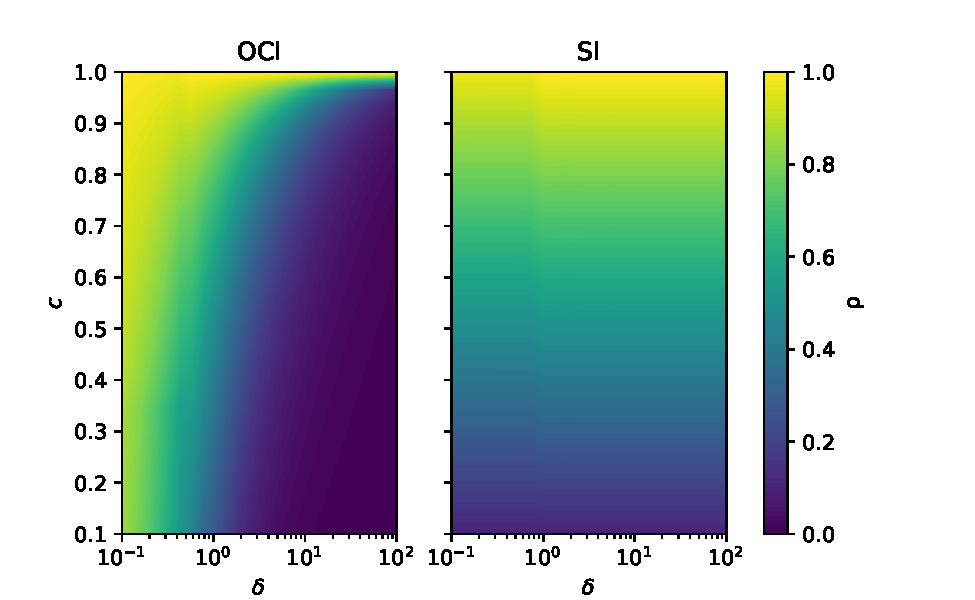
\includegraphics[width=\textwidth]{figures/therefore_figs/ss_specrads.pdf}
    \caption{Spectral radii (${\rho}$) of steady-state OCI (left) and SI (right), where $c$ is the scattering ratio and ${\delta}$ is the cellular optical thickness in mean free paths from Fourier analysis in S$_8$.}
    \label{fig:c2_ss-sepcrad}
\end{figure}

Others have explored OCI as an acceleration scheme for SI \cite{hoagland_hybrid_2021}, a component of a multi-grid solver \cite{man1995multigrid1, man1996multigrid2}, and a solution to the integral transport matrix method \cite{raffi2108pidotscom}.
However, previous investigations of OCI are limited to steady-state computations.

When employing implicit time-differencing schemes (e.g., Crank--Nicholson, backward Euler), each time step involves the solution of a steady-state transport problem with an effective total cross section that includes a time absorption term, proportional to $1/(v \Delta t)$, where $\Delta t$ is time step size and $v$ is radiation speed.
Returning to Fig.~\ref{fig:ss-sepcrad}, the macroscopic total cross section ($\Sigma$) influences both the optical thickness of the cell ($\delta$) and the scattering ratio ($c$), so increasing or decreasing $\Sigma$ will impact convergence behavior.
Spectral radius for both iterative methods decreases as the scattering ratio decreases, but \textit{the spectral radius of OCI also decreases with increasing optical thickness}, which in turn depends on $\Sigma$.
When solving optically thin and highly scattering problems, small increases to $\Sigma$ (and for time-dependent problems, decreases in $\Delta t$ or $v$) may drastically improve the relative performance of OCI compared to SI.
This hypothesis motivates my work, along with evaluating cell-wise algorithms on modern GPU accelerators and exploring higher-order space-time discretization schemes.

\subsection{Preconditioners and Synthetic Acceleration}
\label{c2:precon}

Preconditioners can be used to aid convergence of iterative schemes for the neutron transport equation \cite{adams_fast_2002}.
Often physics-informed preconditioners for transport iterations may be thought of as high-order method solving the full discretized transport equation and a low-order method informing intra-iteration updates to then be used in the next iteration of the high-order problem.
The low-order method is usually some physics-informed problem that is computationally cheaper to solve than the transport problem and model's physical behavior that is difficult for a given operator splitting to converge (e.g., at the diffusive limit, $c\rightarrow1$).

Synthetic acceleration schemes are a common subset of preconditioners for the source iteration operator splitting.
A synthetic acceleration method only \textit{accelerates} convergence to the same solution as transport and is fully consistent with the high-order transport method.
Generally for synthetic acceleration methods the low-order simulation is \textit{driven} by the error between iterations of a transport solve.
Synthetic acceleration techniques for SI include:
boundary projection acceleration \cite{adams_boundary_1988}, 
transport synthetic acceleration \cite{ramone_1997_tsa},
multi-grid methods \cite{man1994parallel},
and the venerable diffusion synthetic acceleration (DSA) \cite{larsen_1983_dsaforsn}, among others.

Diffusion synthetic acceleration is a common preconditioner for the SI operator splitting \cite{adams_fast_2002, alcouffe_1977_dd, coale_2025_dsa}.
It implements a low-order diffusion solve driven by the error between subsequent transport iterations to inform a correction term for the scalar flux, which can in turn be used as the source in a subsequent high-order source iteration.
To make DSA consistent the specific structures of the low-order diffusion solve are governed by the spatial discretization scheme used in the high-order transport simulation.
Larsen's four-step method can be used to yield a DSA scheme that is consistent with spatial discretization; however, the system of equations produced from a Larsen four-step process can be difficult to solve, or form inconsistent schemes for finite elements in higher dimensions \cite{larsen_1982_unconDSA, larsen_1982_unconDSAte, haut_2020_dsa}. 
The Adams--Martin modified four-step process produces consistent schemes with finite element discretization methods \cite{adams_1992_dsadfe}.
Consistent DSA-SI schemes produce rapidly convergent iteration methods where $\rho<c/3$ in homogeneous regions.

Another class of physics-informed preconditioners for the radiation transport equation that do not fall into the sub-category of synthetic acceleration are the moment expansion methods including: second moment (also called Lewis \& Miller methods) \cite{olivier_2024_smoms, lewis_computational_1984, oliver_2025_secondmoment, oliver_phd}, quasi-diffusion \cite{ani_1986_quasidiffusion, goldin_1964_quasidissuion}, and variable Eddington factor \cite{lou_2021_vef, coale_2024_rmomvef} methods.
All of these preconditioners are themselves a set of high-low (HOLO) methods \cite{chacon_2017_holosurvey}.
They still use the same general algorithm as synthetic acceleration where information from the high-order transport solve somehow drives the low-order problem, often with additional physical characteristics (e.g., volumetric material source).
Then, the low-order solution somehow updates information going into the high-order system.
These methods are often inconsistent with the transport equation thus potentially solving a different physical interpretation of the problem physics and converge to a different solution, but they can rapidly converge.

There is less research on preconditioners for OCI when used alone as the primary space-parallel iterative scheme.
OCI itself has previously been used as an acceleration method for source iterations in the forum of either a multi-grid in space solver \cite{kang2000oci, man1994parallel} or a true hybrid scheme (using the same transport mesh) with SI \cite{hoagland_hybrid_2021}.
Rosa and Warsa showed that transport synthetic acceleration (TSA) can resynchronize cells but TSA still requires a potentially expensive sweep operation \cite{tsa2009rosa}.
%Figure \ref{fig:ss_spec_rads} at right shows the spectral radius of TSA-OCI (using no scattering information ($\beta=1$, e.g., a transport sweep between OCI solves).
%Notably for OCI-TSA with $\beta=1$ the method is still potentially unconvergent in the diffusive limit.
%However as $\beta\rightarrow0$ and more scattering physics is included in the low order simulation convergence in the diffusive limit will also be supported.
The search for a non-sweeping---ideally space-parallel or otherwise computationally cheap---preconditioner for OCI to more rapidly converge in the diffusive and thin limits motivates this work.

Yavuz and Larsen described a second moment method they used to accelerate domain decomposed SI sweeps \cite{yavuz_spatial_1989, yavuz_phd}.
They use source iterations within a subdomain and Jacobi iterations to converge incident angular flux between subdomains.
Their method uses a low-order second moment system of equations to inform updates of incident angular flux on the boundaries of each subdomain.
Thus the high-order solver is \textit{not} the SI transport solve but instead the Jacobi iteration.
With their method Yavuz and Larsen showed decreased Jacobi iteration counts for 1D and 2D problems on rectilinear grids \cite{yavuz_spatial_1989, yavuz_1992_2ddd}.
This scheme may aid the convergence of OCI.

While physics-informed preconditioners are often the most robust and applicable to problems of interest preconditioners may be treated more generically from a mathematical perspective.
More generic preconditioners include algebraic multi-grid \cite{southworth_phd}, spatial multi-grid, Jac
Some have anoulouges underlying physics others do not.
The ideas of 
%\section{Considerations for Parallel Computing}
%\label{c2:hpc}


\section{Summary and Relation to Research Questions}

Chapter \ref{chap:therefore_paper} analyzes how the convergence rate of an OCI scheme behaves when used for time-dependent neutron transport computations.
I derive a second-order space-time discretization method from the simple corner balance and multiple balance time discretization schemes and show via Fourier analysis that it is unconditionally stable through time.
Then, I derive and numerically solve the Fourier systems for both OCI and SI splittings of the discretization, showing that small mean-free times improve the spectral radius of OCI more than SI, and that the spectral radius for OCI tends to zero as mean free time gets smaller.
I extend both solvers to be energy dependent (using the multi-group assumption) and implement them on an AMD MI250X using vendor-supplied batched LAPACK solvers.
I show that smaller time steps improve the relative performance of OCI over SI, and, even when OCI requires more iterations to converge a problem, those iterations can be done much faster on a GPU.
This leads to OCI performing better overall than SI on GPUs.
This chapter helps answer research questions:
\begin{itemize}
    \item \emph{RQ1}: How to use software engineering libraries to implement work more efficiently;
    \item \emph{RQ2}: A space-parallel iterative scheme on modern HPC GPUs; and
    \item \emph{RQ3}: How transient behavior impacts convergence of a space-parallel iterative scheme.
\end{itemize}
This work is novel as it is the first time OCI has been implemented on modern GPUs, the first time OCI has been used to solve transient systems, the first time the time-dependent multiple balance approach has been used in conjunction with OCI or the simple corner balance spatial discretization scheme, and the first published use of strided-batched solvers for OCI on the GPU allowing the use of vendor supplied libraries instead of manually scripted GPU kernels.

Chapter \ref{chap:smom_paper} derives a preconditioner to converge OCI faster in the diffusive limit.
I derive a second moment cellular decomposition method in conjunction with a one-cell inversion iteration in an effort to produce a fully space parallel, rapidly convergent, transport iteration.
The method used is based on a preconditioner derived for domain-decomposed problems.
The second moment preconditioner derived in this work does not converge to the same solution as unpreconditioned transport solutions, suggesting inconsistencies between the high and low order equations.
Numerical experiments show the second moment preconditioner rapidly converges in the diffusive limit but does not aid convergence in the optically thin limit.
This chapter helps answer research questions:
\begin{itemize}
    \item \emph{RQ1}: How to use software engineering libraries to implement work more efficiently on modern computing architectures; and
    \item \emph{RQ4}: How to accelerate the space-parallel iterative scheme to converge faster.
\end{itemize}


%Work in this part of my dissertation is in four independent variables in a single angle and spatial dimension.
%While this limits the practical applicability of the exact problems I am solving in this work, the methods may be imp
%In this work I limit to a single spatial dimension.
%This because the problems we are tying to solve (balancing parallelism, time dependence, convergence rate, and searching preconditioners) is dreadfully difficult.
%While the problems I solve are not
%In radiation transport it is common to develop novel numerical methods for simple slab wall problems as the linkage between must be correct in a single \cite{ragusa_robust_2012, larsen_asymptotic_1987, yauz, }
%Without good preconditioning the method described herein has extremely limited applicability to problems of interest which often contain optically thin cells.
%Wil